\chapter{Fake news - seconda parte}

\section{Fake news - seconda parte}

Vi ricordo quello che abbiamo detto nella scorsa lezione. Le fake news sono delle notizie false che sono diffuse massivamente su internet e che possono ingannare, ingenerare delle false convinzioni negli utenti. Il problema delle fake news ha assunto delle dimensioni tali che nell'anno 2017 e anche nel 2018 due importanti enti in ambito europeo hanno deciso di assumere delle posizioni. 

Gli argomenti di oggi:

\begin{itemize}
    \item L'assemblea parlamentare del Consiglio d'Europa, il provvedimento che ha assunto
    \item commissione dell'Unione Europea High Level European Group (HLEG) on Fake News and Online Disinformation che è stato proposto dalla Commissione Europea e che ha elaborato un rapporto.
\end{itemize}

\subsection{L'assemblea parlamentare del Consiglio d'Europa}
Partiamo dal primo argomento, l'assemblea parlamentare del Consiglio d'Europa.
All'inizio del 2017 è stato elaborato un rapporto chiamato Media Online e Giornalismo, sfide e responsabilità. Si tratta della risoluzione numero 2143 del 2017 che è stata pubblicata il 2 febbraio del 2017. 
Di che cosa parla questa risoluzione? 
Parla della prevenzione e della diffusione di notizie false sul web. 

\begin{figure}[ht]
\centering
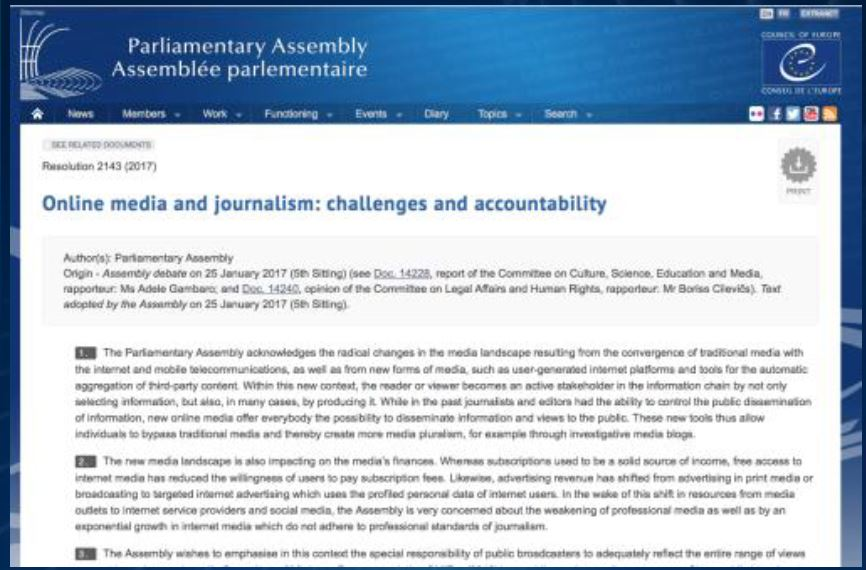
\includegraphics[width=0.8\textwidth]{images/11_lez_fig_01.jpg}
\caption{Pagina ufficiale sul sito con la pubblicazione del testo della risoluzione.}
\label{fig:11_lez_fig_01}
\end{figure}


Nella Figura \ref{fig:11_lez_fig_01} la pagina ufficiale sul sito con la pubblicazione del testo della risoluzione. Non potete leggere perché è soltanto un'immagine, ma potete vedere qual è il sito a cui fare riferimento e dove potete trovare questa risoluzione. \par
Come detto, la risoluzione si chiama Online Media and Journalism Challenges and Uncountability. Sono delle indicazioni di massima di quelle che sono le problematiche legate alla disinformazione online e degli spunti di riflessione e dei suggerimenti agli Stati membri su come è possibile intervenire per cercare di prevenire la diffusione della disinformazione online. \par
Da ricordarsi quando si parla di questo argomento che il web è uno strumento, un ambiente che offre un'infinità di possibilità. \par
Consente una partecipazione attiva del lettore. Il lettore può cercare quelle che sono le informazioni che lo interessano, ma può anche selezionare la produzione delle informazioni in maniera totalmente autonoma. Non solo, il web consente, ha consentito e continua a consentire sempre di più con lo sviluppo della tecnologia ad una informazione non professionale di farsi sentire e quindi la differenza rispetto al passato è enorme. \par
In passato l'informazione considerata tale, il giornalismo considerato tale, era soltanto un'attività di carattere professionale. Questo vuol dire che soltanto persone con una preparazione rispetto alla pubblicazione delle notizie avevano la possibilità concreta di far sentire la loro voce, di raccontare le loro opinioni, di esprimere, di raccontare la vita, il mondo, così come lo vedevano. \par
Con il web invece la possibilità di pubblicare informazioni non è più limitata agli organi tradizionali di informazione professionale, ma è aperta a chiunque. Chiunque con poco, con pochi strumenti, è in grado di pubblicare ciò che ritiene più importante o più opportuno. \par
È anche vero che il web permette di pubblicare informazioni a chiunque, permette anche di conoscere, di prestare attenzione a violazioni di diritti umani che possono essere rilevate in tutto il mondo a cui i media tradizionali a volte prestano scarza attenzione. \par
In questo senso il web è uno strumento formidabile per la diffusione di informazione, maggiore di quello che possono dare gli organi tradizionali. Questo modo di relazionarsi permette anche una mobilitazione di quello che è il cosiddetto popolo del web; le notizie che fanno presa sull'opinione pubblica possono portare a una mobilitazione molto forte di grandi masse di persone anche se non sempre sono basate su fatti reali o su informazioni obiettive. \par
E' capitato, e qui torniamo al tema delle fake news, della disinformazione, delle notizie false, sono capitati spesso episodi nei quali alcune notizie di grande effetto, generalmente corredate da fotografie o da video e da appelli a tutto il mondo tutto vengano ritenute oro colato e questo porta a grandi campagne di opinione, grande libertà di coinvolgere l'opinione pubblica ma anche grande rischio di coinvolgerla su informazioni che in realtà non sono fondate. 

\subsection{Le criticità del web}
Il web ha comunque delle grandi criticità, innanzitutto il tema del finanziamento dei mezzi di informazione. 
Con l'abitudine ad avere a disposizione notizie senza alcun limite, il popolo del web e gli utenti hanno una minore propensione ad abbonarsi agli organi di informazione. Questo però ha una contropartita, la ricerca, la pubblicazione, la selezione di notizie serie, il lavoro del giornalista e il lavoro del professionista è un lavoro appunto che richiede dei finanziamenti, l'organizzazione di un giornale, l'organizzazione di un canale media richiede dei finanziamenti, i giornali tradizionali, i media tradizionali sono stati spesso in parte finanziati dagli Stati ma anche finanziati dagli acquisti.\par
La minor propensione degli utenti ad abbonarsi ai canali di informazione crea un problema di tipo economico di cui bisogna tener conto. \par
Quindi spesso come è possibile finanziare l'informazione sul web? Attraverso la pubblicità e come avviene questo tipo di finanziamento, quali soggetti sono disposti a finanziare siti o blog e quant'altro? 
\subsubsection{Pubblicità e profilazione}
La valutazione sulla importanza di pubblicare una certa pubblicità sul sito dipende dai click, quanti più click un sito riceve, tanto più sarà facile che chi vuole fare pubblicità sia disposto a finanziare quel soggetto. 
Che cosa comporta però il rapporto fra visualizzazione di un sito e pubblicità? Che speso il click fatto sulla pubblicità viene utilizzato per profilare l'utente e si crea un rapporto incestuoso tra la profilazione e l'attività commerciale connessa alla pubblicità. 
%08:25
\subsubsection{Disinformazione e manipolazione sul web}
Possono essere messe in piedi delle campagne che sono realmente dirette a forviare l'opinione pubblica con informazioni false o anche con campagne d'odio. \par 
Abbiamo visto negli anni più recenti il modo in cui sono state impostate due importanti campagne elettorali nel mondo. Trump negli Stati Uniti e Macron in Francia. \par
In entrambi i casi si è fatto un ampio ricorso alle informazioni non tradizionali, a una diffusione di informazioni al di fuori dei canali ufficiali di informazione con strumenti come i social media, con strumenti di messaggistica istantanea, con Twitter. \par
Nel corso della campagna elettorale, più attori hanno diffuso notizie, magari semplicemente commenti, gossip su entrambi i candidati in modo diverso a seconda della campagna elettorale che è capitata. In entrambi i casi l'opinione pubblica è stata scossa e il timore è stato quello che l'opinione pubblica potesse essere distorta, che l'attenzione e la convinzione di tipo politico potesse avere un impatto importante sulla base di questi gossip e messaggi che erano spesso non veri. \par
\subsubsection{obiettivo del Consiglio d'Europa - Contrasto alle fake news}
Alla luce di tutta questa situazione l'obiettivo del Consiglio d'Europa è quello di trovare una maniera di contrastare le fake news perché:
\begin{itemize}
    \item creano allarme sociale
    \item permettono una manipolazione dell'opinione pubblica che può essere pericolosa, che può portare a direzionarla, a portarla verso degli obiettivi non trasparenti.
    \item permette di fare delle campagne d'odio nei confronti di singole persone o di gruppi sociali che possono destabilizzare anche gli Stati
    \item Perché una gestione delle fake news strutturata da parte di chi ha degli obiettivi magari non dichiarati può portare a contrastare quello che è il corretto processo democratico
\end{itemize}

L'informazione professionale secondo il Consiglio d'Europa ha un ruolo determinante come cane da guardia a tutela della imparzialità e della correttezza dell'opinione pubblica. Alla fine delle sue valutazioni quindi il Consiglio d'Europa fa una serie di raccomandazioni a più soggetti, agli Stati membri innanzitutto. 
\begin{itemize}
    \item L'invito è quello a stimolare un dibattito sulle norme possibili da adottare e su dei meccanismi di imprevenzione rispetto alla diffusione della disinformazione online.
    \item a individuare come tracciare gli utenti che violano la legge. E questo tema della tracciabilità è un tema particolarmente delicato. Il tracciamento degli utenti da un lato ha una grande utilità rispetto alla prevenzione o alla repressione di violazioni gravi di legge, dall'altro ingenera il timore che possa esserci un controllo sugli utenti che porterebbe a quella che è la temuta situazione del controllo a distanza. Ricorderete un importante romanzo di Orwell degli anni 80 nel quale si prefigurava proprio un controllo massivo della popolazione attraverso tecnologie informatiche.
    \item Dare un sostegno ai media tradizionali perché anche questi si adeguino agli standards che vengono oggi utilizzati online e facciano attenzione ai contenuti generati dagli utenti in maniera da tenerne conto, raccogliere quello che di buono viene e possano dialogare con gli utenti in maniera da mantenere desta l'attenzione, senza abbassare il livello di guardia rispetto alla correttezza delle informazioni.
    \item considerato questo rapporto fra l'informazione professionale e gli utenti, è importante garantire agli utenti un diritto di replica laddove vi sia da parte dell'informazione professionale un errore. E' anche un obbligo per l'informazione professionale di consentire all'utente la rettifica laddove ci sia appunto una falsa informazione.
    \item formazione rispetto al significato dell'informazione e della corretta informazione che deve partire dalla scuola e che poi deve portare anche a formare i professionisti in maniera adeguata e corretta anche sulle tecnologie attuali, anche sulle modalità di gestione dell'informazione online.
    \item di elaborare dei codici di condotta che possano essere esaminati in collaborazione con i media online e con gli internet service provider, soggetti che sono al di fuori del circuito informativo della raccolta e pubblicazione delle notizie, ma che hanno un ruolo enorme nella diffusione delle notizie e nel tenerle in piedi per lungo tempo.
    \item I proprietari dei siti devono in qualche modo essere responsabilizzati anche rispetto ai contenuti postati da terzi. La regola che fino adesso è stata la regola dominante nel web, è che l'internet service provider che non collaborando alla realizzazione dei contenuti non ha una responsabilità propria per quello che è il contenuto postato. È un po' poco perché il provider è quello che consente all'utente di farsi sentire e quindi in qualche maniera una forma di attenzione, non diciamo controllo, rispetto a quello che viene pubblicato e al fatto che non debba essere in contrasto con i diritti altrui, deve essere mantenuta anche da parte dei provider. 
\end{itemize}


%12:45
\subsubsection{Raccomandazioni per la Federazione Europea dei Giornalisti}
Vi sono nel rapporto anche delle raccomandazioni per la Federazione Europea dei Giornalisti. 

\begin{itemize}
    \item I giornalisti devono fare attenzione ad applicare anche al mondo internet i principi collaudati che sono applicati ai sistemi editoriali e i principi di deontologia.
    \item La pubblicità anche per l'informazione professionale è importante, va gestita e vanno individuati dei rimedi corretti per evitare che con l'uso della pubblicità si arrivi alla violazione di altri diritti come la profilazione. 
\end{itemize}

\subsubsection{Raccomandazioni per l'Associazione Europea dei Fornitori di Servizi Internet}

Il Consiglio d'Europa fa delle raccomandazioni all'Associazione Europea dei Fornitori di Servizi Internet che come abbiamo visto hanno un ruolo determinante nella diffusione dell'informazione. 

\begin{itemize}
    \item I fornitori di servizi internet dovrebbero dotarsi di un codice di deontologia 
    \item dovrebbero permettere agli utenti di segnalare le informazioni non corrette 
    \item dovrebbero anch'essi consentire una rettifica volontaria su richiesta di contenuti non corretti
    \item dovrebbero individuare da un punto di vista tecnico dei meccanismi di allerta e di segnalazione dei trolls.
\end{itemize}

Ecco qui quindi in sintesi quelle che sono le raccomandazioni del Consiglio d'Europa rispetto alla disinformazione online e quindi il più spunto di riflessione per voi. Che cosa raccomanda i governi il Consiglio d'Europa per contrastare le fake news? 

\section{High Level Group on Fake News and Online Disinformation}
La Commissione Europea e il High Level Group on Fake News and Online Disinformation. Cos'è l'High Level Group sulle fake news e disinformazione online? 
\begin{itemize}
    \item 
\end{itemize}

A dicembre 2017 la Commissione Europea ha lanciato l'istituzione del gruppo di lavoro sulle fake news e la disinformazione online.
A gennaio 2018 si è installato, ha cominciato i lavori e a marzo 2018 ha pubblicato il suo rapporto. 
Il tema sono le fake news e in particolare l'individuazione, la definizione, il contrasto alla loro diffusione.

\begin{figure}[h]
\centering
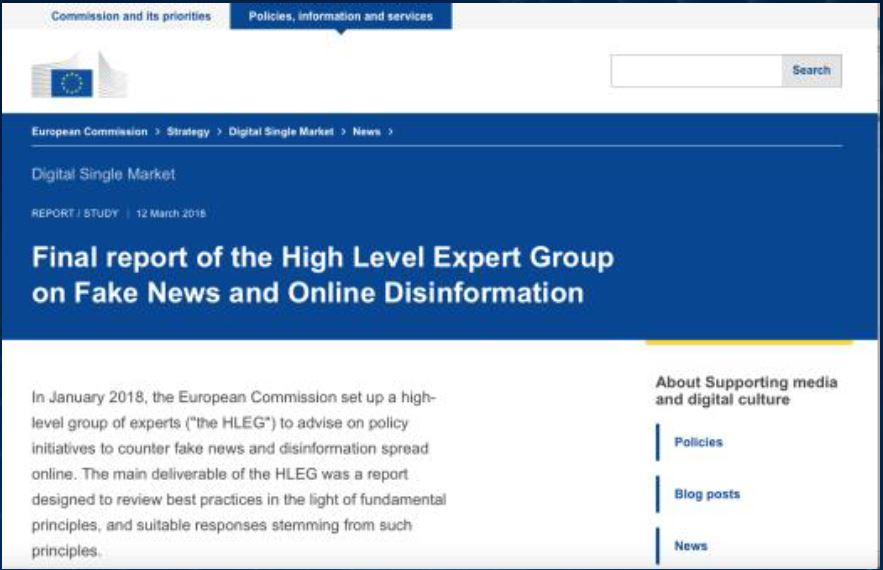
\includegraphics[width=0.9\textwidth]{images/11_lez_fig_02.jpg}
\label{fig: High Level European Group}
\caption{Final Report of the High Level European Group on Fake News and Online Disinformation}
\end{figure}

In Figura \ref{fig: High Level European Group} è per darvi un'idea di quello che è il sito sul quale la Commissione Europea ha pubblicato i lavori della Commissione e soprattutto il rapporto finale del gruppo di esperti sulle fake news e la disinformazione online. \par
I presupposti da cui partono gli esperti per l'elaborazione del loro lavoro è:
\begin{itemize}
    \item il fatto che c'è una stretta interconnessione tra la disinformazione e lo sviluppo dei media digitali
    \item sul web interagiscono una serie di attori diversi, pubblici e privati, commerciali, i media, i cittadini. Ci sono attori individuali e ci sono gruppi di utenti che operano.
\end{itemize}

Questi due elementi sono i presupposti dai quali è partito il gruppo di lavoro per elaborare il suo studio. La Commissione, il gruppo di lavoro, è consapevole che la disinformazione è un fenomeno che va ben oltre il termine fake news.\par
Con questo intende dire che le fake news, secondo il gruppo di esperti, sono solo una fetta della disinformazione online ed è la fetta della quale il gruppo si vuole occupare.\par
Il termine fake news tra il 2017 e il 2018 è diventato talmente importante che per il Collins Dictionary è stato il termine dell'anno 2017 a causa del numero di volte in cui è stato utilizzato sul web. \par
Secondo il gruppo di lavoro della Commissione europea però questo termine è stato utilizzato spesso in modo mistificatorio per indicare anche quello che è semplicemente sgradevole. Non tutto ciò che viene chiamato fake news è veramente fake news. \par 
Che cosa include il gruppo di lavoro nella sua definizione? \par
Innanzitutto fake è ogni informazione falsa, inaccurata o ingannevole che è stata indicata, presentata o promossa per provocare preoccupazione o per ottenere profitto, in ogni caso con intenzionalità. \par
Non è inclusa nella definizione del gruppo di lavoro la creazione e la disseminazione di contenuti illegali, quindi fake nella definizione del gruppo di lavoro non è illegale e come contenuti illegali intendiamo contenuti di carattere diffamatorio, hate speech, incitamento alla violenza. Questo tipo di contenuti illegali sono già regolamentati all'interno dell'Unione europea e degli Stati membri e questa è la ragione per la quale la Commissione ha ritenuto di non prenderli in considerazione.\par
Non rientra nelle fake news la distorsione dei fatti, deliberata ma non ingannevole, ad esempio individuabile nella satira o individuabile nella parodia.\par
Una volta individuati i limiti e i parametri, il gruppo di lavoro ha cercato di individuare i fondamenti per il contrasto alle fake news.
%22:17
\subsection{Fondamenti per il contrasto alle fake news}

Il gruppo di lavoro è consapevole che non esistono soluzioni facili per risolvere il problema, ogni soluzione è comunque complessa e richiede un approfondimento da vari punti di vista. \par

\begin{itemize}
    \item uno degli elementi principali di cui si è tenuto conto è che nell'elaborare delle forme di contrasto e di prevenzione delle fake news, è fondamentale tutelare sempre la libertà di espressione, che è uno dei principi fondanti dell'ordine democratico dei Paesi occidentali
    \item è necessaria una collaborazione di tutti gli stakeholders
    \item è anche necessario un monitoraggio costante dell'evoluzione di ciò che accade sul web
\end{itemize}

Ciò detto, sono stati individuati cinque pilastri. 

\begin{itemize}
    \item Inanzitutto la trasparenza delle notizie, come nascono, come vengono pubblicate
    \item l'alfabetizzazione, che deve essere alfabetizzazione digitale per le generazioni che non sono native digitali, e alfabetizzazione di contenuti, di concetto delle generazioni più giovani
    \item responsabilizzazione di utenti e giornalisti. Da una parte e dall'altra, proprio per il fatto che, come abbiamo visto, sia utenti che giornalisti possono inserire contenuti, è importante che tutti capiscano che devono assumersi delle responsabilità rispetto all'informazione online
    \item la sostenibilità e la diversità dei media all'interno dell'Unione Europea. Nel mondo del 2018 e nel futuro, i media online e offline convivono, e devono continuare a convivere più tipi di media, perché la pluralità è uno degli strumenti essenziali per una informazione libera e corretta. Entrambi questi strumenti, online e offline, devono essere sostenibili da tutti i punti di vista, compreso quello economico
    \item la ricerca. Occorre fare una ricerca continua di quello che è l'impatto delle notizie, di quello che è l'impatto dei media e di quelle che sono le risposte rispetto agli interventi adottati
\end{itemize}

\subsubsection{Raccomandazioni del gruppo di lavoro}
Dopo aver elaborato i cinque pilastri, il gruppo di lavoro ha individuato una serie di raccomandazioni a diversi soggetti. 
Inanzitutto alla la Commissione Europea.
\par
A breve termine: 
\begin{itemize}
    \item La prima raccomandazione, a breve termine, è quella di elaborare dei codici di condotta per tutti gli stakeholders che sono coinvolti
    \item di mettere in piedi un centro di ricerca europeo per affrontare il tema
    \item di promuovere il supporto per dei progetti innovativi che si occupino di questi argomenti
\end{itemize}

A medio-lungo termine:

\begin{itemize}
    \item promuovere delle attività, delle iniziative per l'alfabetizzazione e delle best practices
    \item Promuovere e istituire un safer internet center
    \item individuare e dare agli Stati membri una guida per l'adozione di misure fiscali che consentano la sostenibilità di iniziative valide e corrette per la promozione dell'informazione corretta

\end{itemize}

\subsubsection{Raccomandazioni agli Stati membri}
Il gruppo di lavoro dà delle raccomandazioni agli Stati membri.\par

A breve termine:

\begin{itemize}
    \item individuare dei fondi e strumenti per la ricerca
\end{itemize}

A medio-lungo termine:
\begin{itemize}
    \item promuovere l'alfabetizzazione e la formazione
    \item rafforzamento dell'indipendenza dei media rispetto a forme di pressione di qualunque genere
    \item Sostenibilità finanziaria dei media attraverso forme fiscali, adeguate e corrette, in modo da rendere sostenibile un'informazione corretta e l'innovazione nell'informazione
\end{itemize}


\subsubsection{Raccomandazioni alla società civile}
Da ultimo, la Commissione dà delle raccomandazioni alla società civile.\par
Le raccomandazioni sono  a medio e lungo termine. 

\begin{itemize}
    \item La società civile dovrebbe individuare delle forme di collaborazione alla ricerca anche attraverso l'istituzione di community di cittadini che collaborino
    \item dovrebbero essere elaborate delle piattaforme, dei tools di condivisione degli standard informativi, tali che permettano agli utenti di lavorare in maniera simile a come lavorano coloro che hanno  le piattaforme
    \item dovrebbe stimolare la nascita di New Media pretendendo un'informazione di qualità e operando perché vi sia un corretto fact checking e perché vi sia un approccio etico all'informazione
    
\end{itemize}


Riepilogando, il gruppo di lavoro della Commissione europea, dopo aver individuato il significato di fake news per quello che è l'obiettivo che aveva il gruppo di lavoro, ha dato dei pilastri sui quali fare riferimento e che hanno guidato l'elaborazione del rapporto. Ha poi individuato tutta una serie di azioni da mettere in piedi da parte dei diversi stakeholders interessati al tema, alla Commissione europea, agli stati membri, ai media e alla società civile.\par 
Lo spunto di riflessione per questo argomento. Quali sono i cinque pilastri proposti da Heigh Level Gruop on fake news? \par
Riepiloghiamo gli spunti di riflessione della lezione che abbiamo appena ascoltato:

\begin{itemize}
    \item Cosa raccomanda ai governi il Consiglio d'Europa per contrastare le fake news?
    \item Quali sono i cinque pilastri proposti da Heigh Level Gruop on fake news?
\end{itemize}

Con questa lezione abbiamo concluso l'argomento delle fake news. 
Come ricorderete, questo argomento è stato trattato in due lezioni e questo vi fa capire quanto il tema sia un tema importante. Probabilmente, anche mentre state ascoltando questa lezione, qualcosa è già cambiato. Basti dirvi che a seguito della pubblicazione del rapporto del gruppo di lavoro della Commissione europea, ci sono stati degli eventi importanti che hanno ancora una volta portato all'attenzione del pubblico il problema.\par 

Qual è la dimensione del problema? Proprio nella primavera del 2018, nel marzo-aprile 2018, è scompiato lo scandalo chiamato Cambridge Analytica. \par
Che cosa è successo? È successo che un dubbio che si era posto fin dalla campagna elettorale di Trump, si è iniziato a pensare che forse le fake news sono uno strumento che ha portato a un cambiamento delle decisioni.\par
Il dubbio era stato sollevato, Mark Zuckerberg aveva negato la possibilità di un convolgimento di Facebook rispetto a questo evento. A distanza di un anno e mezzo, invece, questo timore è stato confermato. A primavera, ad aprile del 2018 è emerso che attraverso la società Cambridge Analytica sono stati utilizzati dei profili su Facebook, sono stati violati e sono state diffuse delle informazioni finalizzate proprio a promuovere la posizione di Trump.\par 
Ne è nato uno scandalo enorme, Facebook ha perso moltissimo dal punto di vista economico in borsa e la società Cambridge Analytica è praticamente andata in default per questa ragione. Questo ha portato di nuovo all'attenzione dei governi l'importanza di questo tema. \par
Ancora siamo lontani dal trovare una soluzione, ma certamente va individuata una soluzione senza con questo in alcun modo limitare quello che è il diritto di informazione, la libertà di espressione che deve comunque sempre essere garantita a tutti i cittadini. 